\documentclass[a4paper,12pt]{book}
\usepackage{graphicx}
\usepackage{float}
\usepackage[T1]{fontenc}
\usepackage{hyperref}
\usepackage{adjustbox}
\graphicspath{ {./images/} }
\pagenumbering{gobble}

\hypersetup{
	colorlinks,
	linkcolor=red,
	urlcolor=blue}
	
\begin{document}

\author{Miłosz Wojciechowski}
\title{Telemetry extractor manual}
\date{\today}


\maketitle
\pagebreak
\pagenumbering{arabic}
\renewcommand{\labelenumii}{\arabic{enumi}.\arabic{enumii}}
\tableofcontents
\chapter{Introduction}
This is a manual for the GoPro Telemetry extractor program (download exe file from \href{https://github.com/miloszwojciechowski/Warsaw-model/releases}{github}). As an input it takes an .LRV video file recorded by a GoPro MAX camera. Output of this program is a csv file containing telemetry data (date, timestamp, latitude, longitude and altitude) extracted from the video. Csv file name template is: \verb|<video file name>_telemetry.csv|. \\



Should you need to read about GoPro MAX camera usage, look up its manual: \url{https://gopro.com/content/dam/help/max/manuals/MAX_UM_ENG_REVB.pdf} \\
List of requirements:
\begin{itemize}
	\item GoPro MAX camera
	\item Computer with at least a Windows 10 operating system
\end{itemize}

\chapter{Update GoPro MAX camera}
First of all you need to update your GoPro MAX before recording anything, following steps will show how to do this:
\begin{enumerate}
	\item Download and install the GoPro app on your mobile device (from \href{https://apps.apple.com/us/app/gopro-app/id561350520}{Apple App Store} on iOS or \href{https://play.google.com/store/apps/details?id=com.gopro.smarty&hl=en}{Google Play Store} on Android)
	\item Ensure that your camera is fully charged or with at least \verb|80%| remaining power
	\item Pair your camera with the GoPro app:
	\begin{itemize}
		\item Open GoPro app on your mobile device
		\item \begin{minipage}[t]{\linewidth}
			\raggedright
			\adjustbox{valign=t}{%
				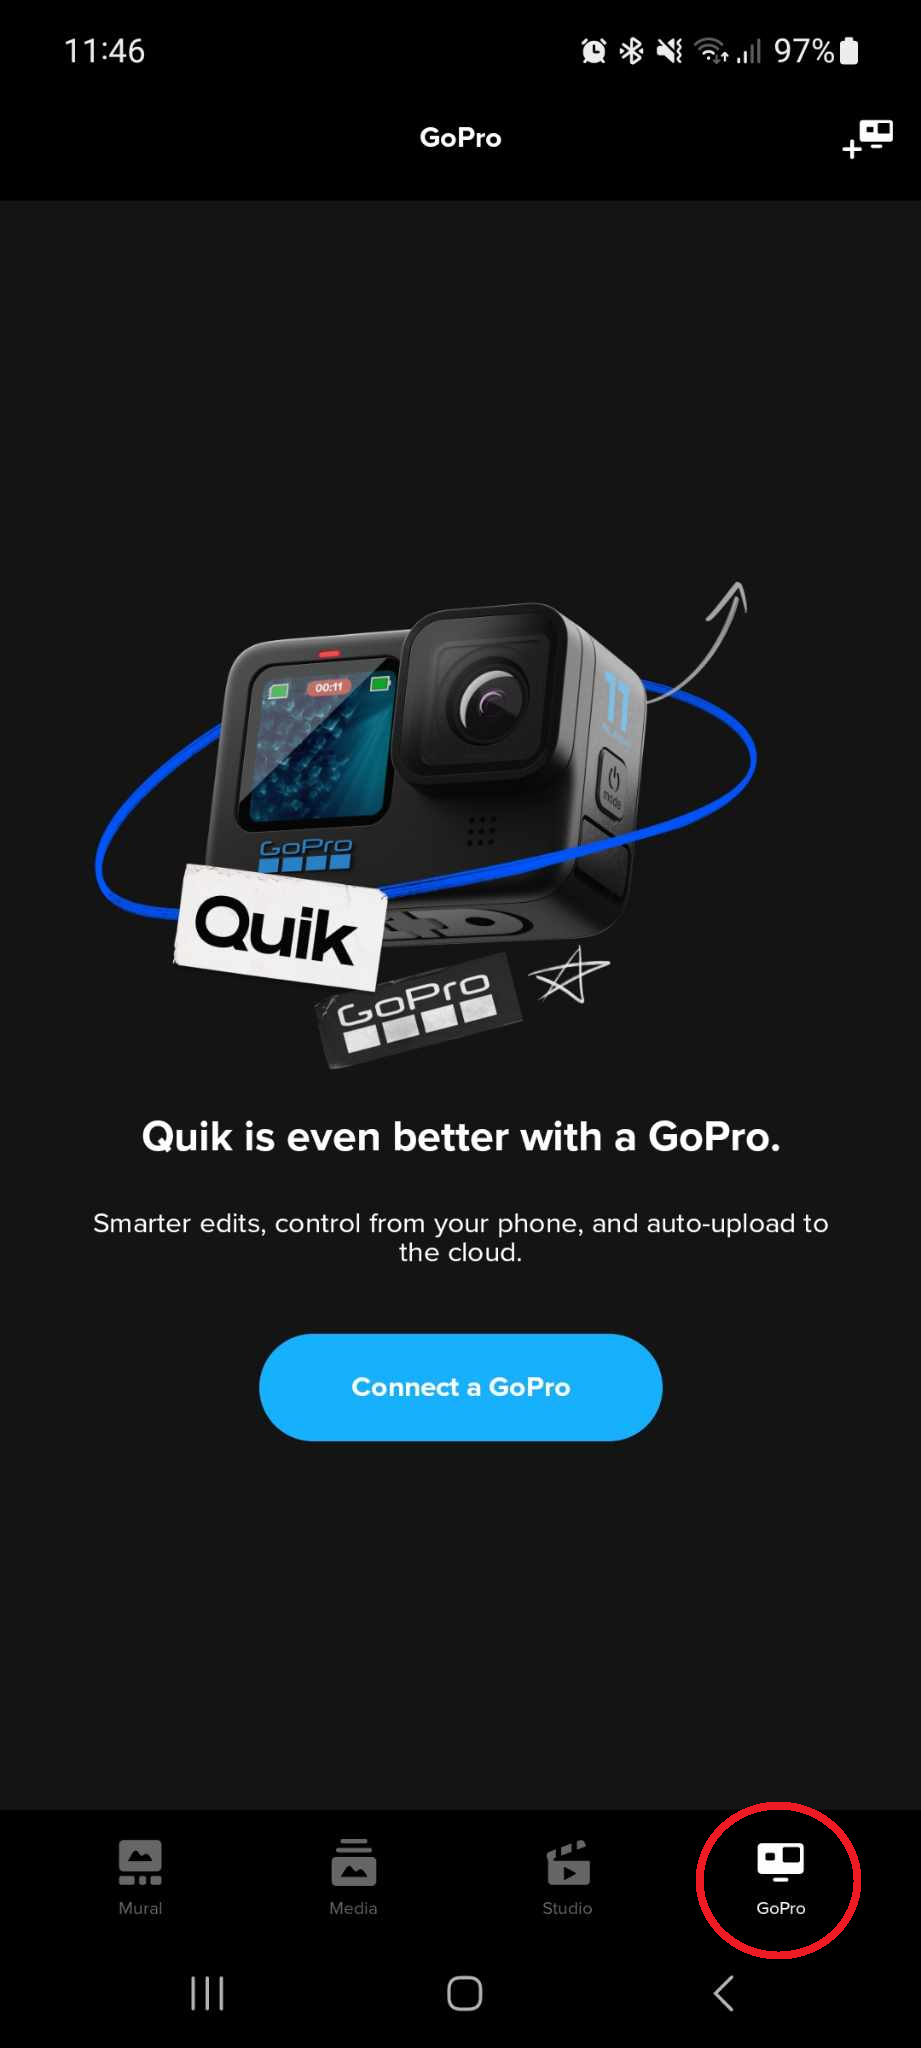
\includegraphics[width=.8\linewidth]{gopro_update1}%
			}		
			\medskip	
		\end{minipage}
		Go to GoPro tab and click Connect a GoPro, choose MAX camera and follow the instructions
		\item If an update is available, the GoPro app will prompt you to update your camera
	\end{itemize}
\end{enumerate}

\chapter{Recording a video}
\section{How to record a video}
\begin{enumerate}
	\item Record a video with your GoPro camera using the following modes:
	\begin{itemize}
		\item Traditional video in HERO or 360 mode
		\item Time Lapse in HERO or 360 mode
	\end{itemize}
	How to use GoPro MAX camera is described in the GoPro MAX manual (link in the introduction). Make sure that you have turned on GPS function otherwise video won't have telemetry data:
	\begin{figure}[H]
		\centering
		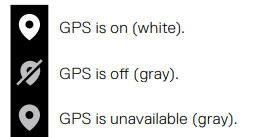
\includegraphics{GoPro_manual_fragment}
		\caption{GoPro Max manual fragment.}
	\end{figure}
	If GPS is off, swipe down to access the Dashboard and Preferences. Click on the Preferences, find option Regional and there turn the GPS On.\\
\end{enumerate}

\section{GoPro video types}
File structure of GoPro Max videos:\\	
GoPro Max creates different types of files during recording, in 360 mode we get:
	\begin{itemize}
		\item .360 file (main video file)
		\item .THM file (thumbnail file)
		\item .LRV file (low-res video file)\\
	\end{itemize}
	In HERO mode (traditional video in 1080p or 1440p) we get:
	\begin{itemize}
		\item .MP4 file (main video file)
		\item .THM file (thumbnail file)
		\item .LRV file (low-res video file)\\
	\end{itemize}
	These files always appear after recording a classical video or a Time Lapse.\\
	
\section{Export camera recordings}
\begin{enumerate}
\item Turn on your GoPro camera.
\item Open your GoPro MAX side panel and connect it to your computer using USB 2.0 to USB-c cable included in a camera set. Information as below should display on the screen:
\begin{figure}[H]
	\centering
	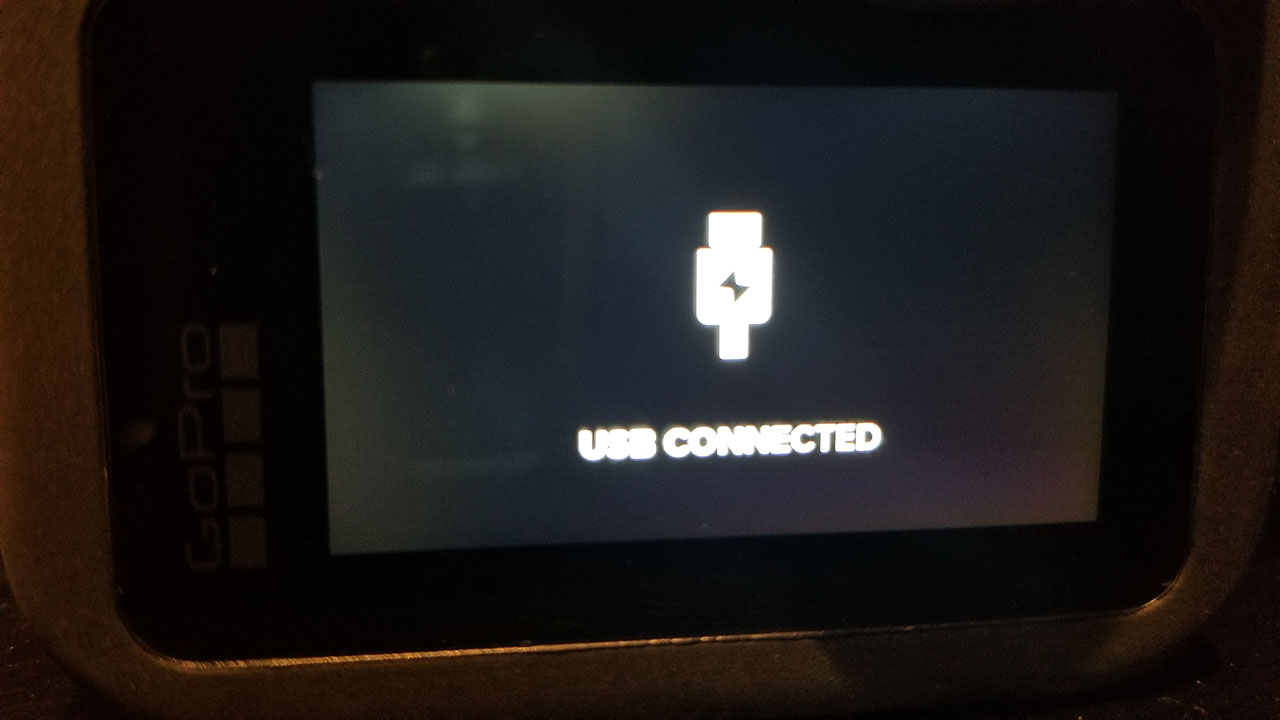
\includegraphics{camera_connected}
	\caption{Successfully connected camera.}
\end{figure} 

\item Now find your connected GoPro camera and navigate through directories:\\

$\textit{GoPro MAX > GoPro MTP Client Disk Volume > DCIM > 100GOPRO}$	\\

Final path should look like this:

\textit{GoPro MAX/GoPro MTP Client Disk Volume/DCIM/100GOPRO}	
\begin{figure}[H]
	\centering
	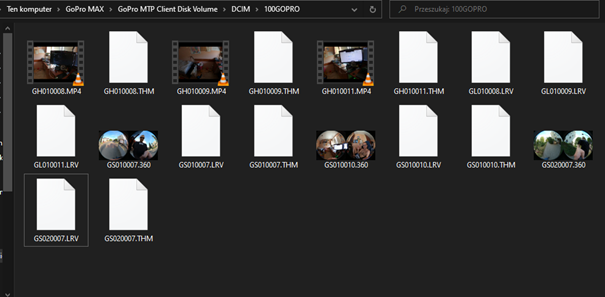
\includegraphics{recording_location}
	\caption{Video files location.}
\end{figure}
\hfill
\item 360 videos’ names and their LRV versions start with GS e.g. GS020007.360, GS020007.LRV.\\

Regular videos’ and their LRV versions’ names start with GH for the former and with GL for the latter e.g. GH010008.MP4, GL010008.LRV. \\
\item Copy videos of your choice and save them on your computer.
\end{enumerate}

\chapter{Run Telemetry-extractor}
\begin{enumerate}
	\item In command prompt either go to GoPro-Telemetry-Extractor location (the one with extractor.exe file) or run program from the default place. Telemetry extractor accepts up to 3 arguments:\\
	\begin{itemize}
		\item path to extractor.exe (if you went to its location in Command Prompt just write extractor.exe e.g "extractor.exe ..."
		\item path to a video file, if a video file is in the same location as extractor.exe only a video file name will be needed e.g. \verb|extractor.exe GS020007.LRV|...
		\item OPTIONAL path to location where telemetry csv file should be generated, if not given a default place for it will be extractor.exe directory
	\end{itemize}
	\item To extract telemetry use .LRV files if possible since this program won't work for files with size bigger than 2GB
	\item As mentioned above you have a few options to run the program:
	\begin{itemize}
		\item Run from completely random place without extractor.exe nor a video file e.g. default Command Prompt directory, command template: \\
		<extractor.exe path> <video file path> <optional telemetry csv generation directory>\\
		e.g.\\
		\verb|S:\GoPro-Telemetry-Extractor\extractor.exe S:\GoPro-videos|\\ \verb|\GS020007.LRV|\\
		
		This will generate telemetry csv file in the extractor.exe location.
		\item Run from extractor.exe directory that doesn't contain video file, command template:\\
		extractor.exe <video file path> <optional telemetry csv generation directory>\\
		e.g.\\
		\verb|extractor.exe S:\GoPro-videos\GS020007.LRV S:\Telemetry\|\\
		
		This will generate telemetry csv file in \verb|S:\Telemetry\| directory.
		\item Run from directory without extractor.exe but with video file, command template:\\
		<extractor.exe path> <video file name> <optional telemetry csv generation directory>\\
		e.g.\\
		\verb|S:\GoPro-Telemetry-Extractor\extractor.exe GS020007.LRV|\\
		
		This will generate telemetry csv file in the extractor.exe location.
		\item Run from extractor.exe directory containing video file, command template:\\
		extractor.exe <video file name> <optional telemetry csv generation directory>\\
		e.g.\\
		\verb|extractor.exe GS020007.LRV S:\Telemetry\|\\
		This will generate telemetry csv file in \verb|S:\Telemetry\| directory.		
	\end{itemize}
\end{enumerate}
 
\end{document}